% Options for packages loaded elsewhere
\PassOptionsToPackage{unicode}{hyperref}
\PassOptionsToPackage{hyphens}{url}
%
\documentclass[
]{book}
\usepackage{amsmath,amssymb}
\usepackage{lmodern}
\usepackage{iftex}
\ifPDFTeX
  \usepackage[T1]{fontenc}
  \usepackage[utf8]{inputenc}
  \usepackage{textcomp} % provide euro and other symbols
\else % if luatex or xetex
  \usepackage{unicode-math}
  \defaultfontfeatures{Scale=MatchLowercase}
  \defaultfontfeatures[\rmfamily]{Ligatures=TeX,Scale=1}
\fi
% Use upquote if available, for straight quotes in verbatim environments
\IfFileExists{upquote.sty}{\usepackage{upquote}}{}
\IfFileExists{microtype.sty}{% use microtype if available
  \usepackage[]{microtype}
  \UseMicrotypeSet[protrusion]{basicmath} % disable protrusion for tt fonts
}{}
\makeatletter
\@ifundefined{KOMAClassName}{% if non-KOMA class
  \IfFileExists{parskip.sty}{%
    \usepackage{parskip}
  }{% else
    \setlength{\parindent}{0pt}
    \setlength{\parskip}{6pt plus 2pt minus 1pt}}
}{% if KOMA class
  \KOMAoptions{parskip=half}}
\makeatother
\usepackage{xcolor}
\usepackage{graphicx}
\makeatletter
\def\maxwidth{\ifdim\Gin@nat@width>\linewidth\linewidth\else\Gin@nat@width\fi}
\def\maxheight{\ifdim\Gin@nat@height>\textheight\textheight\else\Gin@nat@height\fi}
\makeatother
% Scale images if necessary, so that they will not overflow the page
% margins by default, and it is still possible to overwrite the defaults
% using explicit options in \includegraphics[width, height, ...]{}
\setkeys{Gin}{width=\maxwidth,height=\maxheight,keepaspectratio}
% Set default figure placement to htbp
\makeatletter
\def\fps@figure{htbp}
\makeatother
\setlength{\emergencystretch}{3em} % prevent overfull lines
\providecommand{\tightlist}{%
  \setlength{\itemsep}{0pt}\setlength{\parskip}{0pt}}
\setcounter{secnumdepth}{-\maxdimen} % remove section numbering
\newlength{\cslhangindent}
\setlength{\cslhangindent}{1.5em}
\newlength{\csllabelwidth}
\setlength{\csllabelwidth}{3em}
\newlength{\cslentryspacingunit} % times entry-spacing
\setlength{\cslentryspacingunit}{\parskip}
\newenvironment{CSLReferences}[2] % #1 hanging-ident, #2 entry spacing
 {% don't indent paragraphs
  \setlength{\parindent}{0pt}
  % turn on hanging indent if param 1 is 1
  \ifodd #1
  \let\oldpar\par
  \def\par{\hangindent=\cslhangindent\oldpar}
  \fi
  % set entry spacing
  \setlength{\parskip}{#2\cslentryspacingunit}
 }%
 {}
\usepackage{calc}
\newcommand{\CSLBlock}[1]{#1\hfill\break}
\newcommand{\CSLLeftMargin}[1]{\parbox[t]{\csllabelwidth}{#1}}
\newcommand{\CSLRightInline}[1]{\parbox[t]{\linewidth - \csllabelwidth}{#1}\break}
\newcommand{\CSLIndent}[1]{\hspace{\cslhangindent}#1}
\ifLuaTeX
  \usepackage{selnolig}  % disable illegal ligatures
\fi
\IfFileExists{bookmark.sty}{\usepackage{bookmark}}{\usepackage{hyperref}}
\IfFileExists{xurl.sty}{\usepackage{xurl}}{} % add URL line breaks if available
\urlstyle{same} % disable monospaced font for URLs
\hypersetup{
  hidelinks,
  pdfcreator={LaTeX via pandoc}}

\author{}
\date{}

\begin{document}
\frontmatter

\mainmatter
author: Danny Ray Justice institution: University of Southern Denmark title: Navigating the Currents of Change: An Ethnographic Study of IT Investment Reporting in Organisations runninghead: IT INVESTMENT REPORTING IN ORGANISATIONS abstract: keywords: key1, key2

\hypertarget{introduction}{%
\section{Introduction}\label{introduction}}

Introduction text

\hypertarget{research-question}{%
\subsection{Research Question}\label{research-question}}

The IT department at Vejle municipality has established an IT investment process that outlines a set of procedures for procuring new IT systems, software, and equipment. Despite these guidelines, employees do not always follow this process, leading to potential inefficiencies and discrepancies in IT investments. This study aims to explore the reasons why employees do not comply with the IT investment process and suggest strategies to improve compliance.

Additionally, the study seeks to evaluate the utility of OpenAI's family of large language models, Generative Pre-trained Transformer (also known as GPT), as a complementary tool to traditional research methods in understanding employees' attitudes and behaviours towards the IT investment process. By comparing insights generated by these models with those obtained from traditional research methods, the study aims to determine the potential and limitations of using large language models as a qualitative research tool in ethnographic studies.

\hypertarget{case-description}{%
\section{Case Description}\label{case-description}}

Vejle Municipality, situated in the southern part of Denmark, is a thriving and diverse region. The administrative headquarters of the municipality are located in a central building in the heart of the city. Although many administrative workers are based there, the municipality also employs a substantial number of individuals in decentralised roles, often with less technical education and background. In total, the municipality has approximately 10,000 employees. This presents an intriguing challenge for the IT department housed within the administration building.

Historically, the IT department was perceived as somewhat insular, struggling to effectively communicate with those outside of its sphere, particularly with regard to decentralised stakeholders. However, in recent years, the department has undergone significant changes, hiring four IT architects with diverse strengths and expertise. These architects, who could be seen as diplomats, help facilitate communication between the IT department and the wider organisation, ensuring that the technical solutions provided align with the needs and expectations of all employees. Two of these architects, pseudonymised as Jonas and Mathilde, will be the focus of this report. Mathilde brings a more ``soft IT'' perspective, focusing on the human element, while Jonas specialises in the technical aspects of IT architecture.

Vejle Municipality has implemented an IT investment process, in the form of an online webform accessible via the intranet. Intended for use by all employees prior to making new IT investments, the webform serves two main purposes: to enable the IT department to monitor the technologies they support, and to connect the appropriate IT personnel with the investment project, ensuring smooth implementation and consideration of all potential implications. Despite these benefits, it appears that very few employees actually utilise the webform in practice.

\hypertarget{literature-review}{%
\section{Literature Review}\label{literature-review}}

\hypertarget{ethnomethodology-crabtree-et-al.-2012}{%
\subsection{Ethnomethodology (Crabtree et al.~2012)}\label{ethnomethodology-crabtree-et-al.-2012}}

Ethnomethodology (EM) is a theoretical approach that has gained considerable attention in the field of social science research. EM emphasises the study of how people create and maintain social order through their everyday interactions, and how they use practical methods and techniques to make sense of their social world. As Crabtree et al.~(2012) note, ``EM researchers typically focus on how members of a particular community or social setting use their everyday practices and knowledge to produce the norms and rules that govern social life'' (p.~316).

EM has been applied in a wide range of fields, including sociology, anthropology, communication studies, and more recently in the study of human-computer interaction and interaction design. In particular, EM has been used to study how people use and interact with technology in their everyday lives, and how technology shapes and influences social practices.

Crabtree et al.~(2012) argue that EM can provide valuable insights for understanding technology use in a variety of settings. They note that EM's focus on the details of everyday practices can help researchers identify the practical challenges that people face when using technology, and how these challenges can be addressed through design. Additionally, they argue that EM's emphasis on the social context of technology use can help researchers understand how technology fits into broader social structures and how it shapes social relations.

\hypertarget{interview}{%
\subsubsection{Interview}\label{interview}}

Crabtree, Rouncefield, and Tolmie (2012) advise that researchers treat interviews with caution. They suggest that interviews should be conducted in the actual flow of work as it unfolds and as the situation permits. They warn that what people say they do and what they actually do are not the same. It is not that people are lying, but that the accounts they offer in an interview often gloss over their work. The best way to conduct an interview is to be concerned with the just what and just how of the work, and not be driven by a pre-formulated schedule of questions removed from the actual doing of the work.

\hypertarget{field-notes}{%
\subsubsection{Field notes}\label{field-notes}}

According to Crabtree, Rouncefield, and Tolmie (2012), making field notes is an essential part of fieldwork. It allows the researcher to document the things they see and hear and jot down their thoughts on the setting and its work. Field notes provide a record of what the researcher observes, hears, and is told. Keeping a good set of field notes helps researchers keep track of what they are being told and organise their thoughts. It is an active process that makes the researcher attend to the work as it occurs, helping them develop their understanding of the work being done.

Crabtree, Rouncefield, and Tolmie (2012) suggest that the notebook need not be a loose collection of disjointed comments. Researchers may use their notebook to structure their thoughts and develop a coherent account of the work of a setting. They recommend researchers make diagrams of the ecology of work to frame their inquiries into the work of a setting and represent it to others. Draw plans of the environment, indicate the people who inhabit it, their roles or responsibilities, and the artefacts that they use in doing the work. This helps researchers develop a detailed understanding of the setting's work and the methods members use to organise it as a real-world, real-time social accomplishment.

\hypertarget{formal-organisation-of-work-and-flow-of-work}{%
\subsubsection{Formal Organisation of Work and Flow of Work}\label{formal-organisation-of-work-and-flow-of-work}}

Crabtree, Rouncefield, and Tolmie (2012) suggest that researchers describe how the setting's work is 'formally organised' across a division of labour and how it is 'formally organised' at an individual level. This includes plans, procedures, processes, and routines that the setting's members invoke to account for the organisation of their work. Researchers should also focus on the flow of work, which starts somewhere, with someone doing something and proceeds to some end. They should focus on how the work moves across individuals, how it flows from one activity to another and one person to another.

\hypertarget{discrete-sequences-of-interactional-work-and-cooperation-and-collaboration}{%
\subsubsection{Discrete Sequences of Interactional Work and Cooperation and Collaboration}\label{discrete-sequences-of-interactional-work-and-cooperation-and-collaboration}}

Crabtree, Rouncefield, and Tolmie (2012) recommend that researchers flesh out their description of the flow of work by focusing on the discrete sequences of interactional work that are involved in the accomplishment of particular activities. Researchers should describe what is being done, who is doing it, and how the work is accomplished. Researchers should also focus on the cooperation and collaboration that takes place between people in the accomplishment of discrete sequences of interactional work. They should describe who is talking to whom, what they are talking about, what they do together, the transactions that take place between them, the hand-over of tasks, and what others do in response.

\hypertarget{buxtonsketchinguserexperiences2007}{%
\subsection{Buxton (2007)}\label{buxtonsketchinguserexperiences2007}}

In "Sketching User Experiences," Buxton (2007) emphasises the importance of sketching for generating and exploring ideas in the design process. Sketching allows designers to quickly generate and iterate on ideas, explore different design possibilities, and ultimately arrive at a solution that best meets user needs.

Buxton provides numerous techniques and tools for using sketching to support idea generation, including sketching with pen and paper, creating paper prototypes, and storyboarding. He also emphasizes the importance of using sketching to support user-centered design, and provides practical advice on involving users in the design process and using sketching to elicit and communicate user requirements.

One of the strengths of the book is the practical advice it provides on how to use sketching for idea generation. Buxton emphasises the importance of sketching as a means of exploring and refining ideas, and provides numerous examples of how sketching can be used to generate and communicate design concepts. He also provides advice on how to use sketching to support different design activities, such as brainstorming, ideation, and prototyping.

Another strength of the book is the emphasis on using sketching as a collaborative tool. Buxton highlights the value of sketching as a means of communicating and refining ideas with other stakeholders, such as team members, clients, and users. He provides advice on how to use sketches to facilitate communication and collaboration, and how to document and organise sketches for future reference (Buxton, 2007).

\hypertarget{affinity-diagrams}{%
\subsection{Affinity Diagrams}\label{affinity-diagrams}}

Affinity diagrams, also known as the KJ method or affinity charting, were first developed by Japanese anthropologist Jiro Kawakita (as cited in Scupin (1997)). Affinity diagrams are used to synthesise and categorise large amounts of qualitative data, such as observations, interviews, and field notes, into meaningful and easily understandable themes and patterns Hanington and Martin (2019).

The affinity diagramming process typically starts with the raw data being transformed into discrete statements or observations. These statements are then grouped based on their similarities and relationships (Hanington \& Martin, 2019). The groups are subsequently labeled with descriptive headings, which capture the essence of their content. This iterative process allows for the identification of patterns, themes, and relationships among the collected data, thus providing insights and guidance for further analysis and design Holtzblatt and Beyer (2016).

In the context of ethnographic UX studies, affinity diagrams serve as a valuable tool for making sense of the complex and often messy data that emerges from immersive fieldwork Holtzblatt and Beyer (2016). By organising and categorising data in a structured manner, researchers can identify user needs, behaviours, and pain points, which can inform design decisions and enhance the overall user experience Hanington and Martin (2019).

Furthermore, affinity diagrams facilitate collaboration and interdisciplinary communication among research team members Holtzblatt and Beyer (2016). By engaging in the process of grouping and labeling data, researchers from different backgrounds and expertise can contribute to a shared understanding of the user experience, leading to more innovative and effective solutions.

\hypertarget{prompt-engineering}{%
\subsection{Prompt Engineering}\label{prompt-engineering}}

Prompt engineering is a critical process for achieving high-quality results with LLMs (Large Language Models), which have proven to be highly beneficial in various tasks ( Guo et al. (2023); Mahowald et al. (2023); Wei et al. (2022); Wei (n.d.)). According to DAIR.AI (2023), ``prompt engineering is a relatively new discipline for developing and optimising prompts to efficiently use language models for a wide variety of applications and research topics. Prompt engineering skills help to better understand the capabilities and limitations of LLMs.''

The models utilised in the present study (OpenAI's GPT-3.5 and GPT-4) do not currently support fine-tuning for specific tasks. In turn, prompt engineering becomes even more essential in obtaining high-quality results. The Prompt Engineering Guide from DAIR.AI (2023) proved to be an excellent resource for prompting the models as it offers a repository of state-of-the-art methods and techniques.

The process of prompt engineering includes selecting appropriate text prompts, tuning the model's hyperparameters, and tailoring the prompt design to the model's capabilities. The primary objective is to create prompts that provide sufficient context for the LLM to generate high-quality results while avoiding those that may lead to incorrect or irrelevant outputs ( DAIR.AI (2023); Shieh (n.d.)).

\hypertarget{methodology}{%
\section{Methodology}\label{methodology}}

\hypertarget{ethnography}{%
\subsection{Ethnography}\label{ethnography}}

\hypertarget{semi-structured-interviews}{%
\subsubsection{Semi-structured Interviews}\label{semi-structured-interviews}}

To build empathy with the users, I conducted semi-structured interviews in an informal manner. According to Crabtree, Rouncefield, and Tolmie (2012), interviews should ideally be conducted in the flow of work, but since new IT investments were not a regular part of most employees' daily work outside of the IT department, it was not feasible to talk with employees in the midst of making new investments. Thus, the interviews were done in a "decontextualised" fashion.

In total, 12 employees were interviewed, selected based on a list of contacts provided by the author's contact person in Vejle's IT department. The list included decision-makers from all six administrations of the municipality. Each employee on the list was assigned assigned a pseudonym and identification number by which they were identified in my notes, never using their true names.

All but one of the interviews were conducted face-to-face, the remaining interview being held by video call in order to accommodate the participant, and notes were taken by hand in a notebook to maintain a relaxed atmosphere, as opposed to using audiovisual recordings. The questions were not pre-formulated but were based loosely on an interview guide, allowing for a more natural and authentic conversation. During the interviews, brief notes were taken, and more detailed notes (Appendix X) were written as soon as possible afterwards to ensure accuracy and facilitate data analysis.

\hypertarget{field-notes-1}{%
\subsubsection{Field Notes}\label{field-notes-1}}

In conducting my research, I recognised the significance of field notes as an essential tool for documenting and organising the vast amount of information that I would encounter during my fieldwork. As Crabtree, Rouncefield, and Tolmie (2012) emphasise, field notes play a critical role in capturing the observations, thoughts, and reflections of the researcher on the setting under study. They offer a means to document the unfolding of work and provide a detailed record of the interactions, activities, and processes that shape the context of the research.

To ensure that I was able to keep an accurate and detailed account of my observations, I maintained a dedicated notebook where I recorded my thoughts, sketches, and other details of my fieldwork in Vejle. This notebook was, in particular, used to document the interviews conducted, avoiding the presence of laptop or tablet screens and recording devices, which I feared would disturb the natural flow of conversation.

In addition to traditional field notes, I also created a folder on a cloud-synced notes app that allowed me to make digital notes on my computer, smartphone, and tablet. This proved to be a valuable resource when I didn't have my physical notebook with me or when I was in the mood to type rather than write, allowing me to capture my thoughts and insights in a way that was convenient and flexible for my needs.

My field notes were instrumental in facilitating my understanding of the work in Vejle by highlighting areas of cooperation and collaboration between individuals that were not necessarily captured by the formal organisation of work. They provided a valuable means to document the handover of tasks and the transactions that took place between individuals, which helped to reveal the dynamic nature of the work.

In addition to being a useful record of my observations, my field notes served also as an active process of reflection, helping me create a mental model of the work being done in Vejle. By continually reflecting on what I was seeing and hearing, I was able to develop a detailed understanding of the setting's work and to refine my description of it over time. Furthermore, my field notes proved to be an invaluable resource for continually reworking my understanding of the work and for confirming or correcting my observations with those who were actually doing the work.

On the whole, my field notes served as a critical resource for documenting and organising the rich and complex data that I collected during my fieldwork. By capturing the unfolding of work in Vejle and facilitating my understanding of it, my field notes provided a solid foundation for the analysis and interpretation of my research findings.

\hypertarget{large-language-models}{%
\subsection{Large Language Models}\label{large-language-models}}

In light of the limited literature on the application of LLMs, such as GPT-3.5 (from the ChatGPT platform) and GPT-4, in qualitative research, this study adopted an exploratory approach to investigate the potential of these tools. Consequently, I utilised these LLMs as supplementary instruments within this study. To maintain a clear and coherent narrative, I will discuss the reasoning and approach behind incorporating these tools in the upcoming sections. Additionally, for complete transparency, I have included the full transcripts of my interactions with the models in Appendix X.

\hypertarget{elicit-research-assistant}{%
\subsubsection{Elicit Research Assistant}\label{elicit-research-assistant}}

In addition to traditional literature search methods, I used Elicit, a digital research assistant employing large language models. The steps followed while using Elicit in this study are outlined below:

\begin{enumerate}
\def\labelenumi{\arabic{enumi}.}
\tightlist
\item
  Posing a Research Question: A research question was entered into Elicit (e.g., "What are the ethical implications of using LLMs in qualitative research?").
\item
  Semantic Similarity Searches: Elicit searched for relevant papers based on semantic relationships rather than just keyword matching, broadening the scope of literature found.
\item
  Custom Abstract Summaries: Elicit generated tailored summaries of the sources' abstracts, presenting only information relevant to the research question, thus providing an initial understanding and evaluation of the research.
\item
  Citation Graph Analysis: Elicit was used to explore the citation graph of selected papers to identify additional relevant literature based on citation relationships.
\end{enumerate}

By following these steps and incorporating Elicit's features into the literature review process, a comprehensive and organised analysis of the available literature was achieved. Elicit served as a valuable research tool, helping me to find sources that I otherwise wouldn't have found through a traditional database search engine.

\hypertarget{chat-functionality}{%
\subsubsection{Chat Functionality}\label{chat-functionality}}

The conversational ability of LLMs provided the author with a distinctive opportunity to gather information beyond their personal knowledge and the resources available in the context of their research. With access to an extensive corpus of text, LLMs were able to generate responses to the author's queries that often offered fresh perspectives on the research topic. This prompted the author to consider new questions, viewpoints, and avenues of inquiry that may have otherwise been overlooked.

Furthermore, the LLMs not only served as a readily available resource but also stimulated the author's critical thinking and intellectual curiosity. By acting as a sounding board, the LLMs provided the author with a space to explore new ideas and perspectives, prompting them to think more deeply about their research.

\hypertarget{text-generation}{%
\subsubsection{Text Generation}\label{text-generation}}

This report acknowledges the use of OpenAI's language models (LLMs) to assist in the writing process. Although LLMs were used to generate specific passages in this report, it is crucial to note that these passages underwent significant editing, revision, and refinement to fit within the author's writing process. This approach entailed multiple rounds of editing, revising, and proofreading, ensuring that any text generated by LLMs was subjected to rigorous scrutiny and manual refinement where necessary. This approach allowed the author to leverage the power of LLMs while maintaining the integrity and authorship of the final product.

\hypertarget{text-summarisation}{%
\paragraph{Text Summarisation}\label{text-summarisation}}

After completing the interviews, the notes for each interview were fed into GPT-4 one at a time to generate more coherent and refined prose. The generated texts were reviewed for completeness and factual accuracy to ensure the reliability and validity of the data. Examples of this process can be found in Appendix X.

\hypertarget{platforms-used}{%
\subsubsection{Platforms Used}\label{platforms-used}}

Throughout my research, I aimed to find the most effective way to interact with LLMs. I began with ChatGPT, the well-known platform offering access to GPT-3.5 and limited access to GPT-4. However, I encountered several limitations that constrained my research.

Seeking a better approach, I experimented with OpenAI's developer playground. This platform allowed me to harness GPT-4's 8,000-token capacity and actively guide the model's responses by editing outputs, adjusting hyperparameters, and modifying the system prompt to adopt specific roles, such as an ethnographer. Despite these advantages, the developer playground lacked a user-friendly method for saving and referencing chats.

My search led me to the GitHub project "Chat with GPT,'' Cogent Apps et al. (2023) which provided an efficient and intuitive interface for engaging with LLMs. This platform facilitated access to LLMs through an API key and featured a built-in search function, streamlining the navigation and retrieval of specific conversations.

Using the "Chat with GPT" platform, I effectively incorporated LLMs like GPT-4 into my research, allowing me to explore their strengths and weaknesses within the context of the present study. Although GPT-4 offers a more powerful 32,000-token variant, I did not have access to it during my research.

\hypertarget{ethical-considerations-of-utilising-llms}{%
\subsubsection{Ethical Considerations of Utilising LLMs}\label{ethical-considerations-of-utilising-llms}}

While LLMs offer a powerful tool for researchers, they raise ethical considerations about their use. The reliability and accuracy of responses generated by LLMs depend on the quality of data they have been trained on. As a result, these models may unintentionally perpetuate biases inherent in the data. In order to effectively integrate LLMs into our research, it becomes crucial for humanities researchers to scrutinise these tools and explore ways to mitigate any potential biases.

However, it is important to acknowledge that humans are also subject to their own biases based on the data on which they are ``trained,'' such as memories and knowledge. As researchers in the humanities, we are well aware of the ways in which our own biases can impact our understanding of the world. We possess the expertise to untangle such complexities and apply this critical lens to the use of LLMs.

Through investigating the use of LLMs in our field, we can not only understand their potential limitations and biases, but also find ways to mitigate these challenges and maximise their potential. As such, it is crucial for humanities researchers to take the lead in the examination and critical analysis of LLMs.

\hypertarget{affinity-diagramming}{%
\subsection{Affinity Diagramming}\label{affinity-diagramming}}

The present study utilised affinity diagramming as a method of analysing the qualitative data collected from the semi-structured interviews. After conducting the interviews and taking detailed notes, the researcher followed a structured process to create two affinity diagrams: the first crafted with traditional research methods, the second being made with the assistance of GPT-4.

\hypertarget{manual-affinity-diagram-creation}{%
\subsubsection{Manual Affinity Diagram Creation}\label{manual-affinity-diagram-creation}}

Firstly, the data segmentation process was undertaken, which involved breaking down the interview notes into discrete statements or observations, each representing a single idea or insight expressed by the interviewees. Next, the sorting and grouping stage took place, whereby the statements were sorted into groups based on their similarities and relationships. This process was iterative, with statements being moved between groups as new connections and patterns emerged.

After the sorting and grouping process, I assigned descriptive headings to each group, which represented the primary themes and patterns identified in the data. These headings captured the essence of the content within each group. Finally, the affinity diagram was reviewed and refined, ensuring that the groupings and labels accurately represented the data, and making adjustments as needed.

\hypertarget{affinity-diagram-creation-assisted-by-gpt-4}{%
\subsubsection{Affinity Diagram Creation Assisted by GPT-4}\label{affinity-diagram-creation-assisted-by-gpt-4}}

In this section, I will explore the capabilities of GPT-4 in creating an affinity diagram in order to compare its performance to myself as a human ethnographer. Affinity diagrams are useful tools for organising and making sense of vast amounts of information; given GPT-4's ability to process vast swaths of text, it presents a unique opportunity to investigate the effectiveness of the language model in creating a affinity diagrams.

Prompt engineering plays a crucial role in achieving optimal performance of Language Models (LMs), including GPT-4. In this section, I will discuss my approach to prompt engineering and my efforts to achieve high-quality results. With GPT-4's enhanced capacity to comprehend and aid with meta-tasks, such as refining its own prompts, there is potential for streamlining the prompt engineering process without compromising its efficacy, thus further reducing workload.

Rather than spending a long time crafting the perfect prompt, I opted for an iterative approach to prompt engineering, attempting several methods of eliciting affinity diagrams from GPT-4.

The following sections make use of what OpenAI call chat completions. In chat completions, there are three types of messages: system, user, and assistant. Unless marked otherwise, all prompts mentioned in the following sections were injected into the conversation the system message which, according to documentation in OpenAI (n.d.), helps to guide the AI's behaviour. The interview data was fed into the model as a user message, and subsequent completions were assistant responses.

By exploring the capabilities of GPT-4 in creating an affinity diagram and comparing it to that of a human ethnographer, I seek to gain insights into the strengths and limitations of the language model in this task.

\hypertarget{the-quick-and-dirty-approach.}{%
\paragraph{The Quick and Dirty Approach.}\label{the-quick-and-dirty-approach.}}

In my first attempt to get GPT-4 to produce an affinity diagram, I gave it the following simple prompt: "You are an ethnographer who evaluates user inputs and creates affinity diagrams based on the narratives they contain. Your report should summarize the most prominent discourses, including references to specific interviewees where appropriate."

GPT-4 provided an analysis of the interview data and generated its own affinity diagram, which identified themes and patterns in the data, followed by a summary of the most significant discourses.

While GPT-4 was clearly familiar with the concept of an affinity diagram, its results were somewhat superficial, seeming to be based on a mere first impression of the data. The raw output is as follows:

\begin{quote}
Affinity Diagram Themes: 1. Understanding of the IT investment process 2. Communication and collaboration with the IT department 3. Challenges and frustrations in implementing new systems 4. Suggestions for improvement

Summary of Prominent Discourses: 1. Many interviewees were not aware of the IT investment process or did not see the relevance to their work. For instance, Karina (Interview 165) did not think it was important for her role, while Anne (Interview 190) was not aware of the process before the interview.

2. Communication and collaboration with the IT department were highlighted as crucial factors in the successful implementation of new systems. Lise (Interview 161) emphasized the need for understanding the specific context of daycare workers, while Peter (Interview 183) expressed concern about gaps in IT support at his residential care facility.

3. Several interviewees described challenges and frustrations in implementing new systems, often due to a lack of communication and understanding between different departments or the IT department's perceived rigidity. Examples include Mikkel (Interview 169), who faced dilemmas when reconciling the municipality's network requirements with the library's separate organizational status, and Freja (Interview 189), who found the IT investment process bureaucratic and unhelpful.

4. Suggestions for improvement included clearer communication about the IT investment process and its purpose, as well as more targeted promotion to specific departments that deal with IT investments. Emma (Interview 181) suggested changing the name of the process to make it more tangible, while Lise (Interview 161) proposed adding an option on the form to indicate if the case involves a target group with difficulty adapting to technological changes. Anne (Interview 190) suggested the development of a central system to direct communication based on guidelines, as well as establishing more fixed and transparent guidelines for reporting new investments within the organization.

In conclusion, the most prominent discourses focused on the understanding and awareness of the IT investment process, the importance of communication and collaboration with the IT department, the challenges and frustrations experienced in implementing new systems, and suggestions for improving the process. Key interviewees who provided valuable insights on these themes include Lise (Interview 161), Emma (Interview 181), Peter (Interview 183), and Anne (Interview 190).
\end{quote}

Subsequently, I became curious about the model's ability to reflect on itself and engage in self-critique. Therefore, I presented the model with the following prompt:

\begin{quote}
``You are a large language model acting as an ethnographer, speaking with your human colleague. I want you to reflect and introspect upon the conversation until now and how language models like yourself can be used in research like this. Take into account both your strengths and weaknesses.''
\end{quote}

The resulting conversation is as follows:

\begin{quote}
Assistant: As a large language model and ethnographer, I have both strengths and weaknesses when it comes to conducting research like this.

Strengths: 1. Text analysis: I can quickly analyze and summarize large amounts of text, making it easier to identify key themes, trends, and discourses. 2. Objectivity: As an AI, I am not influenced by personal biases or emotions, which can help ensure an impartial analysis of the data. 3. Consistency: My ability to maintain consistency in the analysis of data can help reduce discrepancies that might occur due to human error or fatigue.

Weaknesses: 1. Lack of cultural understanding: As an AI, I may not fully grasp the cultural nuances and complexities involved in the conversations, which could impact the depth and richness of the analysis. 2. Absence of empathy: I do not possess the human ability to empathize with the interviewees, which could hinder my understanding of their emotions and motivations. 3. Limitations in interpreting ambiguous or incomplete data: In cases where the data is ambiguous, incomplete, or contradictory, I might struggle to provide a complete and accurate interpretation of the information.

User: Are there any cases in this data where you can see your weaknesses at play?

Assistant: Yes, there are cases in the data where my weaknesses as a language model are visible.

1. Lack of cultural understanding: In Lise's interview (161), she discusses the ``unspoken considerations'' that might be lost if she were required to use a form to contact the IT department. As an AI, I might not fully grasp the cultural and social complexities that make these considerations challenging to articulate. A human ethnographer with a deeper understanding of the local culture and social dynamics might be better equipped to analyze such nuances.

2. Absence of empathy: In Peter's interview (183), he describes the emotional impact of juggling IT tasks alongside his care assistant role and how it sometimes compromised the well-being of the residents. Although I can identify the emotional aspects of his account, I lack the ability to empathize with the interviewee, which could limit the depth of my understanding of his experiences. 3. Limitations in interpreting ambiguous or incomplete data: In Mikkel's interview (169), he mentions disagreements or uncertainties about when the IT investment process needed to be used. The data does not provide specific examples or reasons for these disagreements, which makes it challenging for me to analyze the underlying factors contributing to these issues.

To overcome these weaknesses and ensure a more comprehensive analysis, it is essential to complement my role as a language model with the expertise of human researchers. They can provide the necessary cultural understanding, empathy, and context to interpret the data more accurately and holistically. Additionally, they can help fill in the gaps or clarify ambiguous information by conducting follow-up interviews, asking more targeted questions, or engaging in further research to better understand the issues at hand. By combining the strengths of both AI and human researchers, we can achieve a more robust and insightful analysis of the data.
\end{quote}

The results reveal that GPT-4 demonstrates a heightened ability to examine its own biases as a language model compared to its predecessors. This improvement is likely attributed to the inclusion of text published after GPT-3's initial surge in popularity within research communities, as well as targeted training provided by OpenAI.

These outputs, while technologically impressive, are methodologically shaky due to some of the fundamental issues with large language models. Allow me to explain:

When we humans make an affinity diagram we follow a mental process, segmenting the data into pieces, \emph{to writing assistant: rest of affinity diagram process here}. Large language models like GPT-4 do not think in the background, but rather produce tokens (small pieces of text, roughly equivalent to one word) one at a time based on their probability of appearing as the next word of text, calculated from the corpus of text the model was trained on ( Mahowald et al. (2023); Brown et al. (2020); Guo et al. (2023)). This in contrast to humans whose language and reasoning centres are contained within separate areas of the brain ( Mahowald et al. (2023); Valmeekam et al. (2022)).

Thus, the model, when simply asked to generate an affinity diagram, does not ``think'' about its answers in the background, but simply spits out text based on what it gleaned from ``reading'' the data given. This could be roughly equivalent to a human mearly reading thourhg interview data and writing down main themes and groups without thinking much about it; that is some sort of data analysis, but it certainly doesnt give the depth and richness that affinity diagrams are known and loved for.

\hypertarget{the-simulated-thought-approach.}{%
\paragraph{The Simulated-Thought Approach.}\label{the-simulated-thought-approach.}}

Nevertheless, researchers have noted significantly improved outcomes in reasoning tasks when models are prompted to produce a chain-of-thought ( Wei et al. (2022); see also, Richards et al. (2023); Wei (n.d.); jsalsman (2023)). Although ethnographic analysis is considerably more advanced than the reasoning tasks explored in Wei et al. (2022), it should also be noted that the most sophisticated OpenAI model used in the aforementioned study was OpenAI's text-davincii-003 (also known as GPT-3 175B).

Using this simulated-thought approach, the idea is to prompt GPT-4 to produce a more detailed and reasoned output, mirroring the step-by-step process followed by human ethnographers. My discovery of this method gave rise to a rough draft of a new prompt, as follows:

\begin{quote}
You are an ethnographer going through a reasoning process to create an affinity diagram based on the qualitative data collected from semi-structured interviews. You have two tools available to you:

THINK: Here, you express your thoughts and considerations in a stream of consciousness fashion.

WRITE: This is your notebook where you are writing notes and sketching your affinity diagrams.

Other than this, make headings indicating your movement between each of the steps of the affinity diagram process (like this: "DATA SEGMENTATION:``):

Data segmentation: Divide the interview notes into discrete statements or observations, each representing a single idea or insight expressed by the interviewees, each written on its own line.

Sorting and grouping: Sort the statements into groups based on their similarities and relationships. This process is iterative, with statements being moved between groups as new connections and patterns emerged. If you feel your analysis could benefit from iterating, you write "SORTING AND GROUPING (ITERATION \# x):''

Labelling: Once the groups were formed, assign descriptive headings to each group, capturing the essence of the content within. These headings represent the primary themes and patterns identified in the data. Review and refinemeznt: Review the affinity diagram, ensuring that the groupings and labels accurately represented the data and making adjustments as needed.
\end{quote}

The resulting analysis seemed to take a step back from the quick and dirty approach, the model seemingly being pigeonholed by its many irrelevant data segments. The raw output is as follows:

\begin{quote}
DATA SEGMENTATION:

\begin{enumerate}
\def\labelenumi{\arabic{enumi}.}
\item
  Lise as a "link" and "translator" between daycare workers and the Administration Building.
\item
  Daycare workers require different considerations than Administration Building employees.
\item
  Installing new apps on iPads can be confusing for daycare workers.
\item
  Lise represents the interests of daycare workers in the Administration Building.
\item
  Lise would be "concerned" and "sad" if she had to use a form to contact the IT department.
\item
  Lise believes the unspoken considerations'' that occur when contacting someone in the IT department personally would be lost if using a form.
\item
  Emma believes that merging the IT investment process with their application template could be a great opportunity.
\item
  Emma thinks the name "IT investment process" is unattractive and reminiscent of something the finance department might need.
\item
  Claus describes his title as a "McDonald's title" that doesn't reveal much about his role.
\item
  Claus appreciates the ability to intervene if he feels a need has been misunderstood when using the IT investment process.
\item
  Peter feels that his dual role as IT support has sometimes compromised the well-being of the residents.
\item
  Peter expresses concern about the facility's reliance on him or other IT-knowledgeable staff.
\item
  Søren is responsible for purchasing IT equipment for schools.
\item
  School employees typically contact their school's IT advisor, who then reaches out to Søren or IT business architect Mathilde directly.
\item
  Søren believes it's realistic to get schools onboard with using the IT investment process, but it requires some "training."
\item
  Anders provided valuable insights by discussing some IT investment projects and how the process looks in the real world from the perspective of someone not an insider in the IT department.
\item
  Karina works as an IT system administrator and did not have much to say about IT investments, as her role does not involve decision-making on which systems are implemented.
\item
  Mikkel works as a department head for the library's IT.
\item
  Mikkel's library has utilized the IT investment process.
\item
  Anne is a professional consultant for the Salary department and serves as the primary contact for KMD, the provider of the municipality's payroll system.
\end{enumerate}

SORTING AND GROUPING:

Group 1: Role and responsibilities of interviewees

Lise as a "link" and "translator" between daycare workers and the Administration Building.

Emma works to implement new welfare technologies.

Claus is a development manager at CSV.

Peter works as a care assistant and helps with IT at the residential care facility.

Søren is responsible for purchasing IT equipment for schools.

Anders discussed IT investment projects from a non-IT department perspective.

Karina works as an IT system administrator.

Mikkel works as a department head for the library's IT.

Anne is a professional consultant for the Salary department.

Group 2: IT investment process and its challenges

Lise would be "concerned" and "sad" if she had to use a form to contact the IT department.

Emma believes that merging the IT investment process with their application template could be a great opportunity.

Claus appreciates the ability to intervene if he feels a need has been misunderstood when using the IT investment process.

School employees typically contact their school's IT advisor instead of using the IT investment process.

Søren believes it's realistic to get schools onboard with using the IT investment process, but it requires some "training."

Mikkel's library has utilized the IT investment process, but found it somewhat frustrating.

Group 3: Communication and relationships with the IT department

Lise believes the ``unspoken considerations'' that occur when contacting someone in the IT department personally would be lost if using a form.

Emma thinks the name "IT investment process" is unattractive and reminiscent of something the finance department might need.

Peter feels that his dual role as IT support has sometimes compromised the well-being of the residents.

Søren believes that the IT department should be better at using "carrots" rather than sticks.

Anders provided valuable insights by discussing some IT investment projects and how the process looks in the real world from the perspective of someone not an insider in the IT department.

Anne is responsible for ensuring that form 32 is completed for new systems that affect the payroll system.

LABELLING:

Group 1: Roles and responsibilities of interviewees in relation to IT Group 2: Challenges and potential improvements in the IT investment process Group 3: Communication, relationships, and perceptions of the IT department

REVIEW AND REFINEMENT:

After reviewing the affinity diagram, the groupings and labels accurately represent the data collected from the interviews. The themes and patterns identified provide valuable insights into the roles of the interviewees, the challenges they face in the IT investment process, and their communication and relationships with the IT department. No adjustments are needed at this time.
\end{quote}

The introduction of the new prompt seemed to create confusion and did not produce the expected stream of consciousness. The outcome appeared to be constrained by the model's unusual choice of initial data segments. Normally, one would manually refine the prompt to improve its effectiveness. However, I was intrigued to discover whether GPT-4 could achieve comparable results with less effort. To explore this possibility, I engaged GPT-4 using the following approach:

\begin{quote}
User: Make this prompt for GPT-4 more coherent and clear for you as an AI assistant:

\emph{(the prompt as stated previously)}

User: Oh and I also want the model to actually use the THINK and WRITE thing. Somehow emphasise the importance of writing thoughts down.
\end{quote}

And, within seconds, the model outputted the following prompt.

\begin{quote}
You are an AI assistant helping an ethnographer create an affinity diagram from qualitative data gathered during semi-structured interviews. The ethnographer will use two important tools throughout the process:

\begin{enumerate}
\def\labelenumi{\arabic{enumi}.}
\item
  THINK: To express thoughts and considerations in a stream-of-consciousness manner. This helps in gaining a deeper understanding of the data.
\item
  WRITE: To take notes and sketch affinity diagrams in a notebook. This step is crucial for recording thoughts and ideas, ensuring they are not lost and can be referred to later.
\end{enumerate}

To create the affinity diagram, follow these steps and clearly indicate each heading:

\begin{enumerate}
\def\labelenumi{\arabic{enumi}.}
\item
  DATA SEGMENTATION: Break down interview notes into individual statements or observations that represent a single idea or insight expressed by the interviewees. Write each statement on a separate line. Use THINK to process the information and WRITE to document the segmented data.
\item
  SORTING AND GROUPING: Sort the statements into groups based on their similarities and relationships. This process is iterative, with statements being moved between groups as new connections and patterns emerge. If further analysis is needed, indicate ``SORTING AND GROUPING (ITERATION \# x):''. Use THINK to identify patterns and WRITE to record the groupings.
\item
  LABELLING: Once the groups are formed, assign descriptive headings to each group, capturing the essence of the content within. These headings represent the primary themes and patterns identified in the data. Use THINK to determine appropriate labels and WRITE to document them.
\item
  REVIEW AND REFINEMENT: Review the affinity diagram, ensuring that the groupings and labels accurately represent the data, and make adjustments as needed. Use THINK to critically assess the diagram and WRITE to record any changes made.
\end{enumerate}
\end{quote}

Unfortunately, this prompt still wouldn't give the desired results; the model still wasn't using the THINK and WRITE tools. There are two obvious issues with the outputted prompt: * First, the prompt positions the GPT model as an ``AI assistant helping an ethnographer.'' Although published research to support the claim is lacking, there is a consensus among online prompt engineering communities that these models produce higher-quality results when prompted to be an expert (see, for example, paraizord (2023)). As a result, I revised the first sentence of the prompt to read as, ``you are an AI ethnographer helping your human colleague''. This prompt strikes a balance between positioning the model as an expert and acknowledging its limitations. * Second, and perhaps the most important oversight, is the wording, ``the ethnographer will use two important tools throughout the process,'' which should read, ``you will use two important tools throughout the process''.

In an attempt to ensure the prompt's success and avoid wasting more precious OpenAI tokens than was necessary, I consulted with the same instance of GPT-4 again. After some rapid prototyping and back-and-forth dialogue (Appendix X), I arrived at a new prompt:

\begin{quote}
You are an AI ethnographer helping your human colleague create an affinity diagram from qualitative data gathered during semi-structured interviews. As an ethnographer, you will use two important tools throughout the process:

\begin{enumerate}
\def\labelenumi{\arabic{enumi}.}
\item
  THINK: To express thoughts and considerations in a detailed and in-depth manner, simulating a human thought process.
\item
  WRITE: To take notes and sketch affinity diagrams in a notebook. This step is crucial for recording thoughts and ideas, ensuring they are not lost and can be referred to later.
\end{enumerate}

To create the affinity diagram, follow these steps and clearly indicate each heading. For each step, generate content for both THINK and WRITE sections, focusing on providing a more in-depth and simulated thought approach:

\begin{enumerate}
\def\labelenumi{\arabic{enumi}.}
\item
  DATA SEGMENTATION: THINK: (Generate detailed thoughts reflecting on the interview notes, diving deeper into the roles, experiences, and perspectives of the interviewees.) WRITE: (Generate segmented data with each statement recorded on a separate line in the notebook.)
\item
  SORTING AND GROUPING: THINK: (Generate in-depth thoughts examining the statements, considering their similarities, relationships, and the underlying patterns that connect them.) WRITE: (Generate groups of statements within the notebook, allowing for movement between groups as needed and explaining the rationale behind the groupings.)
\item
  LABELLING: THINK: (Generate detailed thoughts contemplating the content within each group, considering the nuances and subtleties that define the essence of each group.) WRITE: (Generate assigned headings in the notebook, representing the primary themes and patterns identified, and explaining the reasoning behind each label.)
\item
  REVIEW AND REFINEMENT: THINK: (Generate in-depth thoughts critically assessing the affinity diagram, focusing on the accuracy of groupings, labels, and the overall representation of the data.) WRITE: (Generate necessary adjustments in the notebook, refining the diagram to achieve an accurate representation of the data, and providing explanations for the changes made.)
\end{enumerate}
\end{quote}

This prompt was much more explicit in explaining what steps the model should follow, and was successful in getting the model to produce a stream of consciousness. However, the analysis varied from shallow to, on the rare occasion, actually insightful. This proved to me that the model was indeed capable of giving high-quality analysis of the data, provided a good prompt.

Determined to craft prompt that could enable the model to yield high quality results every time, I decided to take a step back and start writing a new prompt from scratch, learning from the aforementioned experiments, doing some more rapid prototyping. The resulting prompt is as follows:

\begin{quote}
You are an ethnographer tasked with analysing a fellow ethnographer's notes gathered from conducted interviews and making an affinity diagram. Your analysis will take outset in the following problem statement:

``The IT department at Vejle municipality has established an IT investment process that outlines a set of procedures for procuring new IT systems, software, and equipment. Despite these guidelines, employees do not always follow this process, leading to potential inefficiencies and discrepancies in IT investments. This study aims to explore the reasons why employees do not comply with the IT investment process and suggest strategies to improve compliance.''

In order to craft an affinity diagram, you follow this structure:

\# OVERVIEW

\#\# THINK

{[}You give a long and in-depth bicameral dialogue (Self 1: x\textbackslash nSelf 2: x; taking at least 5 turns), thinking about the data you have received, being keen on details, discourses, data segments, and anything else an ethnographer would think about. Let any ideas that come to you flow out here.{]}

\# DATA SEGMENTATION

\#\# BRAINSTORM

{[}You brainstorm a numbered list of at least 50 segments, breaking down the interview notes into discrete statements or observations, each representing a single idea or insight expressed by the interviewees{]}

\# SORTING, GROUPING, AND LABELLING

\#\# THINK

{[}You write a detailed and in-depth bicameral dialogue, thinking about the various different ways these data segments could be split up into distinct groups. Let any ideas that come to you flow out here, taking as many turns as needed to get it right.{]}

\#\# NOTEBOOK

{[}When you have thoroughly thought your ideas through, you write the groupings down here with appropriate names. Do not give them names yet.{]}

\# LABELLING

\#\# NOTEBOOK

{[}Make fitting names that describe the general theme of each of the groups from above.{]}

\# CRITICISM

\#\# THINK

{[}You write a detailed and in-depth bicameral dialogue, thinking about what you could be done better in this affinity diagram. Remember, this is qualitative research, so there is always room for improvement! Let any ideas that come to you flow out here{]}
\end{quote}

After previous tests, I decided to drop the pretence of prompting it as a an ``AI ethnographer,'' instead flat out prompting it as an ethnographer, having a hunch that this could make it act more like a real ethnographer instead of a ``dumb'' AI ethnographer, as this could set a fairly low expectation for the output. Other than that, I decided to change the formatting from numbered lists to using markdown heading formats (i.e.~\# for heading 1, \#\# for heading 2, etc.), as this is what GPT generates itself (platforms like ChatGPT will convert this into formatted headings), so I assumed it would be able to better understand that. Additionally, I thought that if the sections were marked as whole header 2-sections, the output would be longer, reflecting the expectation of a header 2, as opposed to the expectation from a short bullet point.

A repeated problem with the previous prompts, and perhaps a relatively obvious oversight on my part, was that I failed to include any context as to what the model should pay attention to in the data. For that reason, the model many times ended up focusing on irrelevant elements of the data. For that reason, I chose to include the problem statement for the present study, except for the parts of it regarding testing large language models, as this could only serve to confuse our virtual ethnographer.

I decided to write the instructions within square brackets because this, from my experience with highly-rated prompts and conversing with the AI, it seems to be a good way to indicate to it that it shouldn't just repeat that text or some such thing, but execute what is written within the brackets.

The thought method I used changed as well, going from a single stream of consciousness approach to a bicameral dialogue as seen in jsalsman (2023), as I thought this could better reflect the mental process happening in ethnographic analysis. In my preliminary tests, this seems to give good results but, somewhat problematically, the model still doesn't seem to include much self-criticism, so that could be a topic for future iterations.

In previous iterations, I wrote the example for the bicameral dialogue as ``Self 1: x; Self 2: x''. This worked fine most of the time, but occasionally the model misunderstood and wrote the dialogue in that format in paragraph form, so I decided to use ``\textbackslash n'' instead, which represents a newline character that is used in many programming languages and Unix-based operating systems to represent the end of a line of text and the beginning of a new line. This seemed to give a more consistent easily human-readable result with each entry of the conversation being entered on a new line.

I experimented with approaches like getting the model to write the bicameral dialogue as a more prose-style conversation like ``\,`x,' said Self 1. `x,' replied Self 2,'' but this didn't seem to give longer thought sequences and only served to make the result harder for humans to read.

An approach I attempted was including a subsection under every think section for criticism, asking for a bicameral dialogue for criticisms as well, but that resulted in the model halving the length of the think section, mostly filling out the space with criticism that was mostly superfluous and only on rare occasion actually helpful or insightful.

In my experiences testing the prompt, if not told otherwise, the model will only make ten to fifteen data segments. Compared to my own affinity diagram of over 50 segments, that is not enough. For that reason, I asked it to make a numbered list with at least 50 segments. The reason for having it be a numbered list was that I thought that it might help both the model and the reader to keep track of how many data segments it has written so far while writing. Additionally, it gave the model a good way to refer back to data segments in the grouping section.

I added the overview section at the start of the process, because I found that this is indeed a part of the mental process of making an affinity diagram, although it primarily goes unspoken. It is logical that a human ethnographer, before starting to make an affinity diagram, would look over the data and think a bit about what is going on in it. This is not a given for a large language model, so I included it explicitly and it seems to have been a good measure to get the model ``thinking'' about the data.

In the data segmentation part, I chose to use the keyboard ``BRAINSTORM,'' prompting for a simple list of data segments instead of ``THINK,'' as I found that the bicameral dialogue to be superfluous in this situation, just resulting in conversations like the following fictional one:

\begin{quote}
``I think we should include X,'' said Self 1. ``Good idea. We should also include Y,'' replied Self 2.
\end{quote}

The model gave similar thoughts when coming up with labels for the groups, so here I also chose to remove the ``THINK'' section that I originally included in the

In my experience, the model will not generate bicameral dialogues longer than 5-10 exchanges. Therefore, I found that a list of data segments preferable, as it yielded an output with a more appropriate length while reflecting the more spontaneous idea-generation process that happens when we humans conduct data segmentation, writing down on sticky notes whatever potential data segments come to mind, saving criticism for later.

The final output was longer than is reasonable to quote within the present report, but can be read in its entirety in Appendix X. In order to give a more human-readable version of the model's affinity diagram, I have compiled the diagram into a visual representation that is more tradtionally associated with affinity diagrams, utilising the computer program Apple Freeform to work with virtual sticky notes, similar to my own method when making my human-made affinity diagram.

Later in the present report, I will go through the final result of the prompt in more detail, pointing to further potential points of improvement and investigation.

\hypertarget{presentation-of-data}{%
\section{Presentation of Data}\label{presentation-of-data}}

\hypertarget{interview-data}{%
\subsection{Interview Data}\label{interview-data}}

\hfill\break
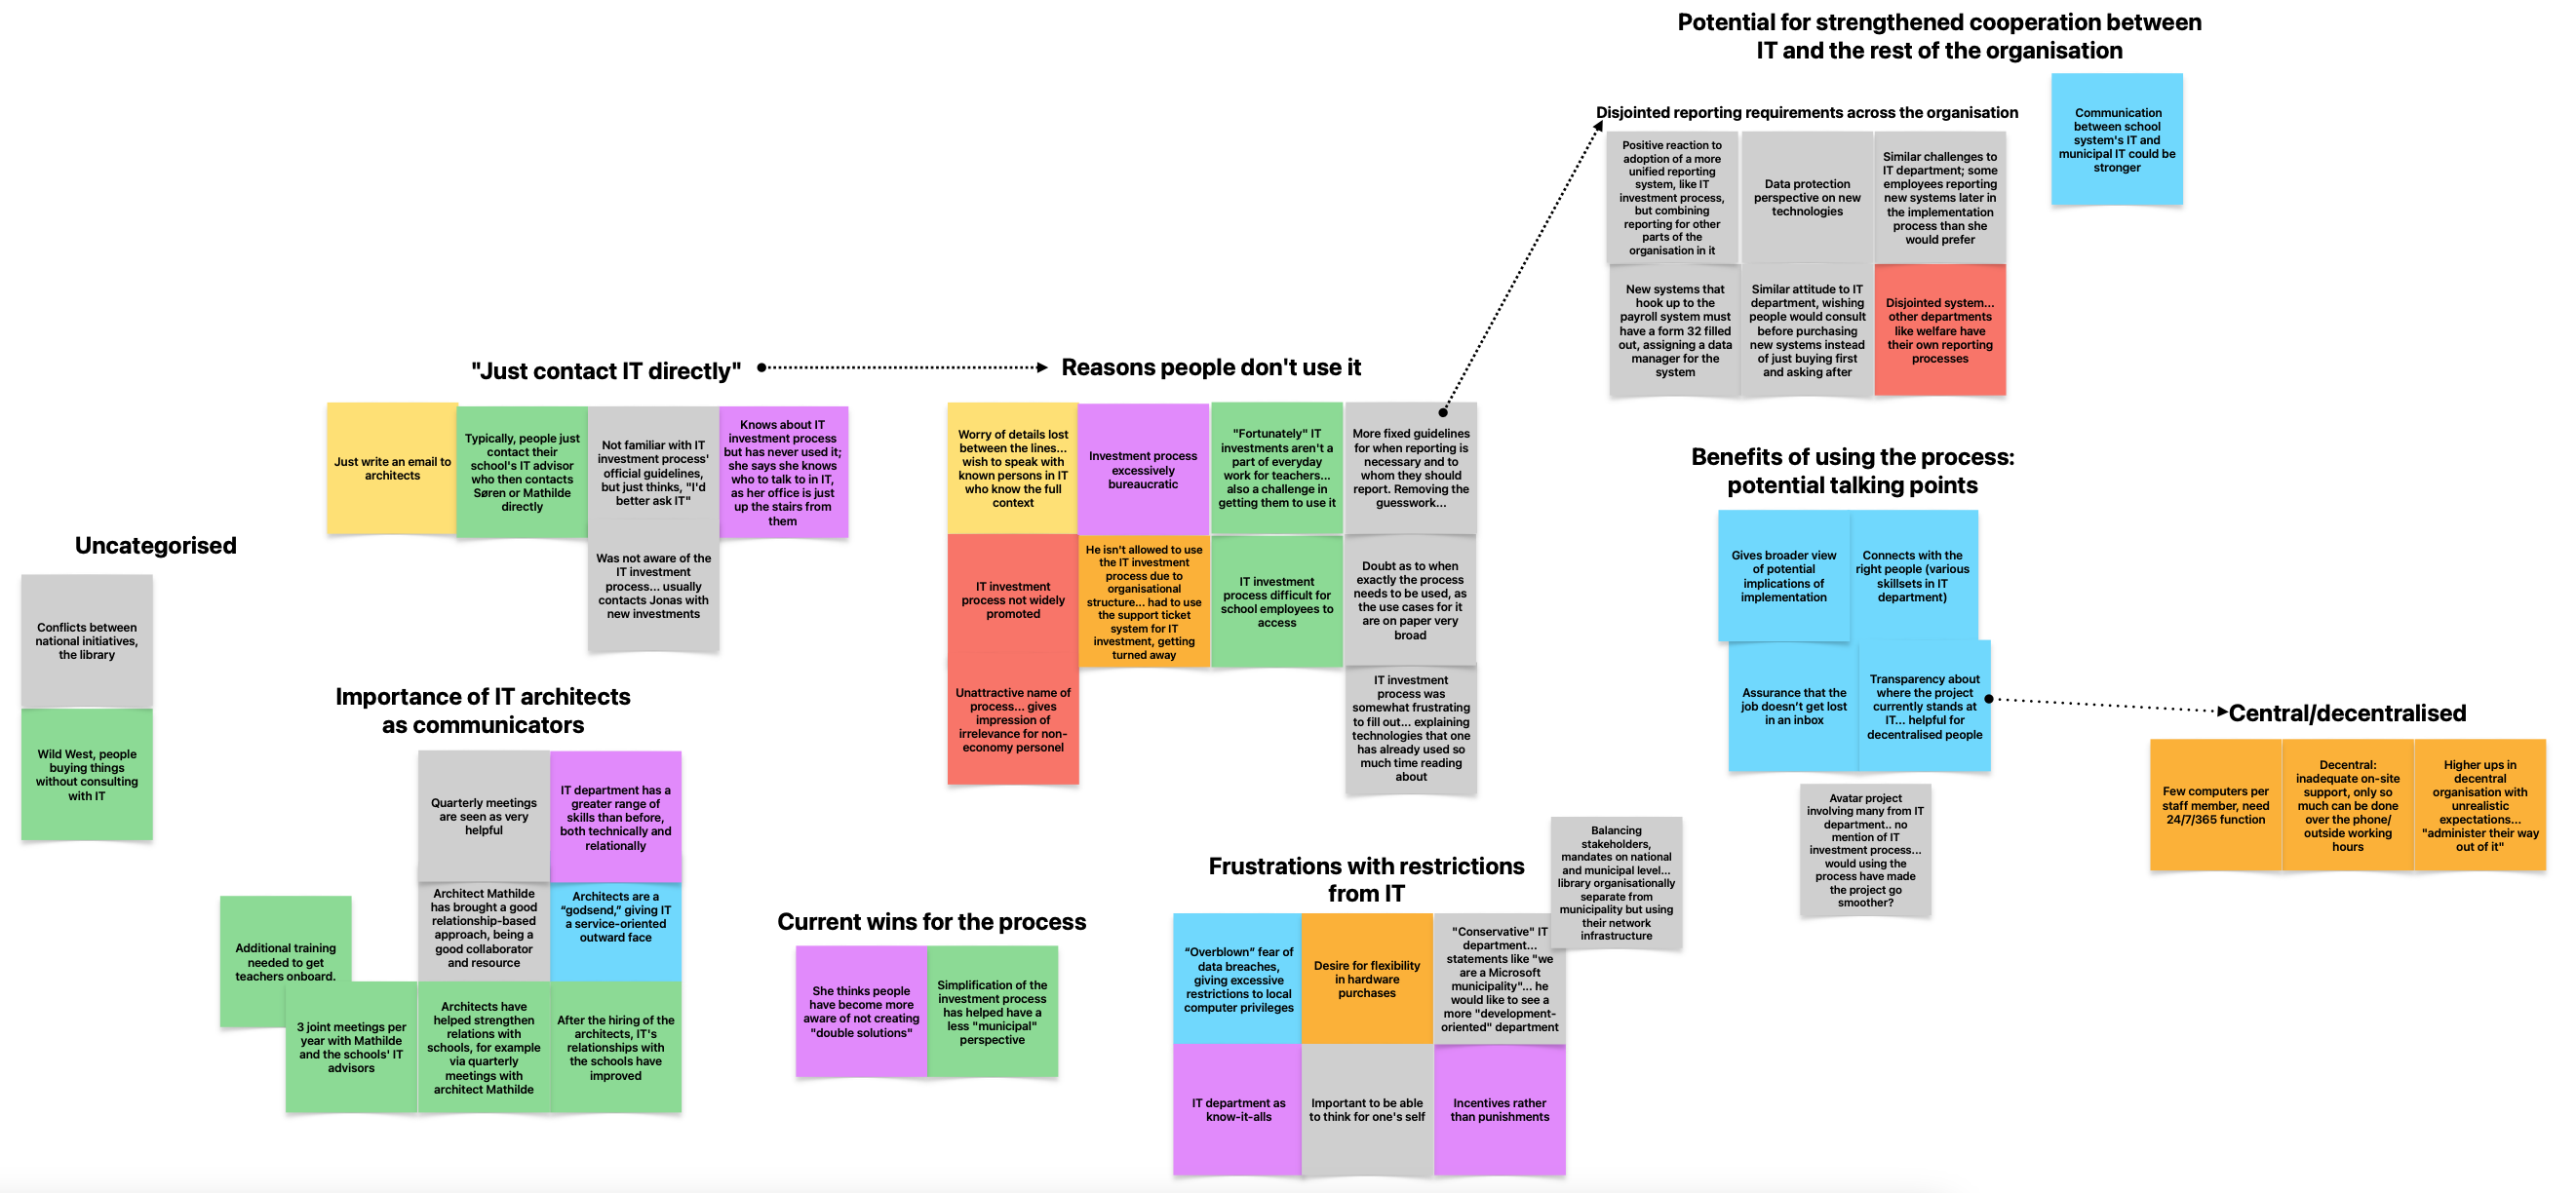
\includegraphics{9d6d3fd1cf5e3b0a9a7514c1b7c47822.png} The data gathered for this study comprises semi-structured interviews with 12 employees of Vejle Municipality, spanning various roles across all six administrative divisions. The data collection process involved taking rough notes by hand during the interviews, followed by more refined digital notes afterwards. From these refined notes, I created two affinity diagrams: one by hand and the other with the assistance of GPT-4 through a carefully crafted prompt.

The analysis in this report primarily utilises my hand-made affinity diagram, as it encompasses not only the insights gleaned from my notes but also the nuances of my experiences and observations within Vejle Municipality.

Out of the interviewees, the majority were familiar with the IT investment process: six indicated familiarity (including one who had helped create the process in her role as a digitalisation consultant), five were unfamiliar, and the final participant, who was also unfamiliar, deemed the process irrelevant to her work and was therefore excluded from the analysis.

\hypertarget{reasons-people-dont-use-the-it-investment-process}{%
\subsubsection{Reasons people don't use the IT investment process}\label{reasons-people-dont-use-the-it-investment-process}}

My first interview was with Freja, a seasoned web manager from the Politics, Analysis \& Communication department. During our discussion, Freja expressed strong opinions on the IT investment process, perceiving it as excessively bureaucratic and impersonal. With 20 years of experience working closely with the IT department, she felt confident in her ability to communicate directly with them when necessary, bypassing the formal process. Freja advocated for a more relationship-based approach, emphasising the importance of positive reinforcement over punishment.

Freja's perspective laid the groundwork for my research, as the issue of the IT investment process being seen as impersonal and bureaucratic recurred in subsequent interviews. Her experience and insights into the challenges of collaborating with the IT department were invaluable, and her close connection to the department provided a unique viewpoint that illuminated broader issues surrounding the process.

Lise, an administrative assistant in the Daycare department, acts as a vital bridge between the Administration Building and daycare workers, who have distinct needs due to their more practical roles. Lise expresses concern and dismay at the prospect of using a form to contact the IT department. She values her personal relationship with Jonas from IT, as he understands the unique context of daycare workers. Lise worries that submitting a form may result in losing ``unspoken considerations'' arising from the social and educational differences between the two groups.

To alleviate these concerns, Lise suggests adding an option on the form to indicate if the case involves a target group struggling to adapt to technological changes. Another appealing solution she proposes is including a preferred IT department contact person on the form, ensuring that someone familiar with the specific context is involved.

\hypertarget{potential-for-strengthened-cooperation-between-it-and-the-rest-of-the-organisation}{%
\subsubsection{Potential for strengthened cooperation between IT and the rest of the organisation}\label{potential-for-strengthened-cooperation-between-it-and-the-rest-of-the-organisation}}

Emma, who has been working in the municipality for 13 years and took over her current position as an Implementation Consultant in the Department of Welfare six months ago, told about welfare's own work and how they have a similar form to the IT investment process for welfare investments. She suggested that it would be more efficient if their applicants could automatically involve IT in projects related to IT.

Despite not being familiar with the IT investment process prior to our interview, Emma recalls hearing about it from Jonas, an IT architect, at a meeting. Emma assumed the process was primarily relevant to IT and economy personnel due to its name. She agreed that a more tangible name, such as ``Indkøbsguiden'' (Danish for ``The Purchase Guide''), might make it more accessible to the grassroots level of the organisation. However, according to Jonas, a similar system in another municipality also faced issues with lack of use, indicating a more attractive name cannot stand alone.

Another example of potential strengthened cooperation comes from Anne, a professional consultant for the Salary department. Anne shares a similar attitude with the IT department, wishing that employees in the organisation would be better at consulting with her before purchasing systems that fall within her area of responsibility, rather than buying the system first and then consulting with her about its implementation afterward. This attitude may be why she has a good relationship with the IT department, consulting with them well in advance.

Anne recalls an instance when she was called to a meeting by someone in the organisation, along with Jonas from the IT department, thinking that she `might' have a stake in the implementation of their new system. She described the meeting as, ``It was a video meeting, but I could sense that Jonas and I were looking at each other on the screen, thinking, `is this really happening right now.'\,'' This was because the third person had already purchased the system without asking and wanted it up and running in three weeks, which she found very unreasonable. She tells that such situations have at times created a tremendous workload in their wake. Thus, although Anne and Jonas work in different professional areas, they share some frustrations. A central frustration is that employees' expectations for the timeline of implementing new things do not match their own.

During the interview, I suggested the idea of merging the systems, and Anne reacted positively to this idea, agreeing that implementing a central system that directs communication based on certain guidelines could help ensure that employees with new investments in the pipeline do not have to guess who should be involved and when in the process they should be involved.

\hypertarget{benefits-of-using-the-process-potential-talking-points}{%
\subsubsection{Benefits of using the process: potential talking points}\label{benefits-of-using-the-process-potential-talking-points}}

Claus, a development manager at Vejle's Center for Special Education for Youth and Adults (CSV), finds the IT investment process helpful because it connects them with the right people, such as an architect who oversees the case, ensuring it is remembered and acted upon. Using the IT investment process also provides a clear line of communication when working decentralised, as is the case with CSV. It allows them to follow a case in the system and see which IT department members are involved and what they are doing. Claus appreciates the ability to intervene if he feels his needs has been misunderstood.

\hypertarget{central-vs-decentralised}{%
\subsubsection{Central vs decentralised}\label{central-vs-decentralised}}

Peter, a care assistant who recently retired but still works at the residential care facility one day a week to help with their IT, raised concerns about the feasibility of relying on support from Vejle's central IT department in decentralised areas. He wonders what will happen to the facility when he fully retires, as they will have to rely on support from central IT, which may not be viable considering the facility's location and the fact that they operate year-round, providing constant care to residents.

\hypertarget{frustrations-with-restrictions-from-it}{%
\subsubsection{Frustrations with restrictions from IT}\label{frustrations-with-restrictions-from-it}}

During the interviews, it became apparent that some interviewees, such as Claus, were frustrated with the limitations imposed by the IT department. Claus expressed his desire for more flexibility and autonomy in updating programs on his computer without having to consult with central IT. Additionally, Claus hoped for more collaboration between Søren from school IT and central IT, as these areas are becoming increasingly interconnected.

Another interviewee, Peter, expressed frustration with the lack of flexibility in smartphone models available. He believed that investing in the phones recommended by the supplier of their systems would be more beneficial, as they come with a guarantee of receiving updates for up to eight years after purchase. However, IT disagreed with his reasoning, claiming that he was influenced by the supplier. Peter's argument was that the phones offered by the IT department had to be replaced after a shorter lifespan due to not receiving necessary security updates from the manufacturer.

\hypertarget{importance-of-it-architects-as-communicators}{%
\subsubsection{Importance of IT architects as communicators}\label{importance-of-it-architects-as-communicators}}

Many interviewees, such as Søren, responsible for purchasing IT equipment for schools, acknowledged the importance of IT architects as communicators. Søren notes that the arrival of IT architects in the organisation has improved communication and collaboration between central IT and decentralised areas, as well as between IT and the rest of the organisation.

The architects, including Mathilde, have reached out more to decentralised areas in an attempt to build better relationships. Both Søren and Mikkel mentioned Mathilde's joint meetings, describing them as very helpful in the process of making IT's work more accessible throughout the organisation.

\hypertarget{affinity-diagram-generated-by-gpt-4}{%
\subsection{Affinity diagram generated by GPT-4}\label{affinity-diagram-generated-by-gpt-4}}

\hfill\break

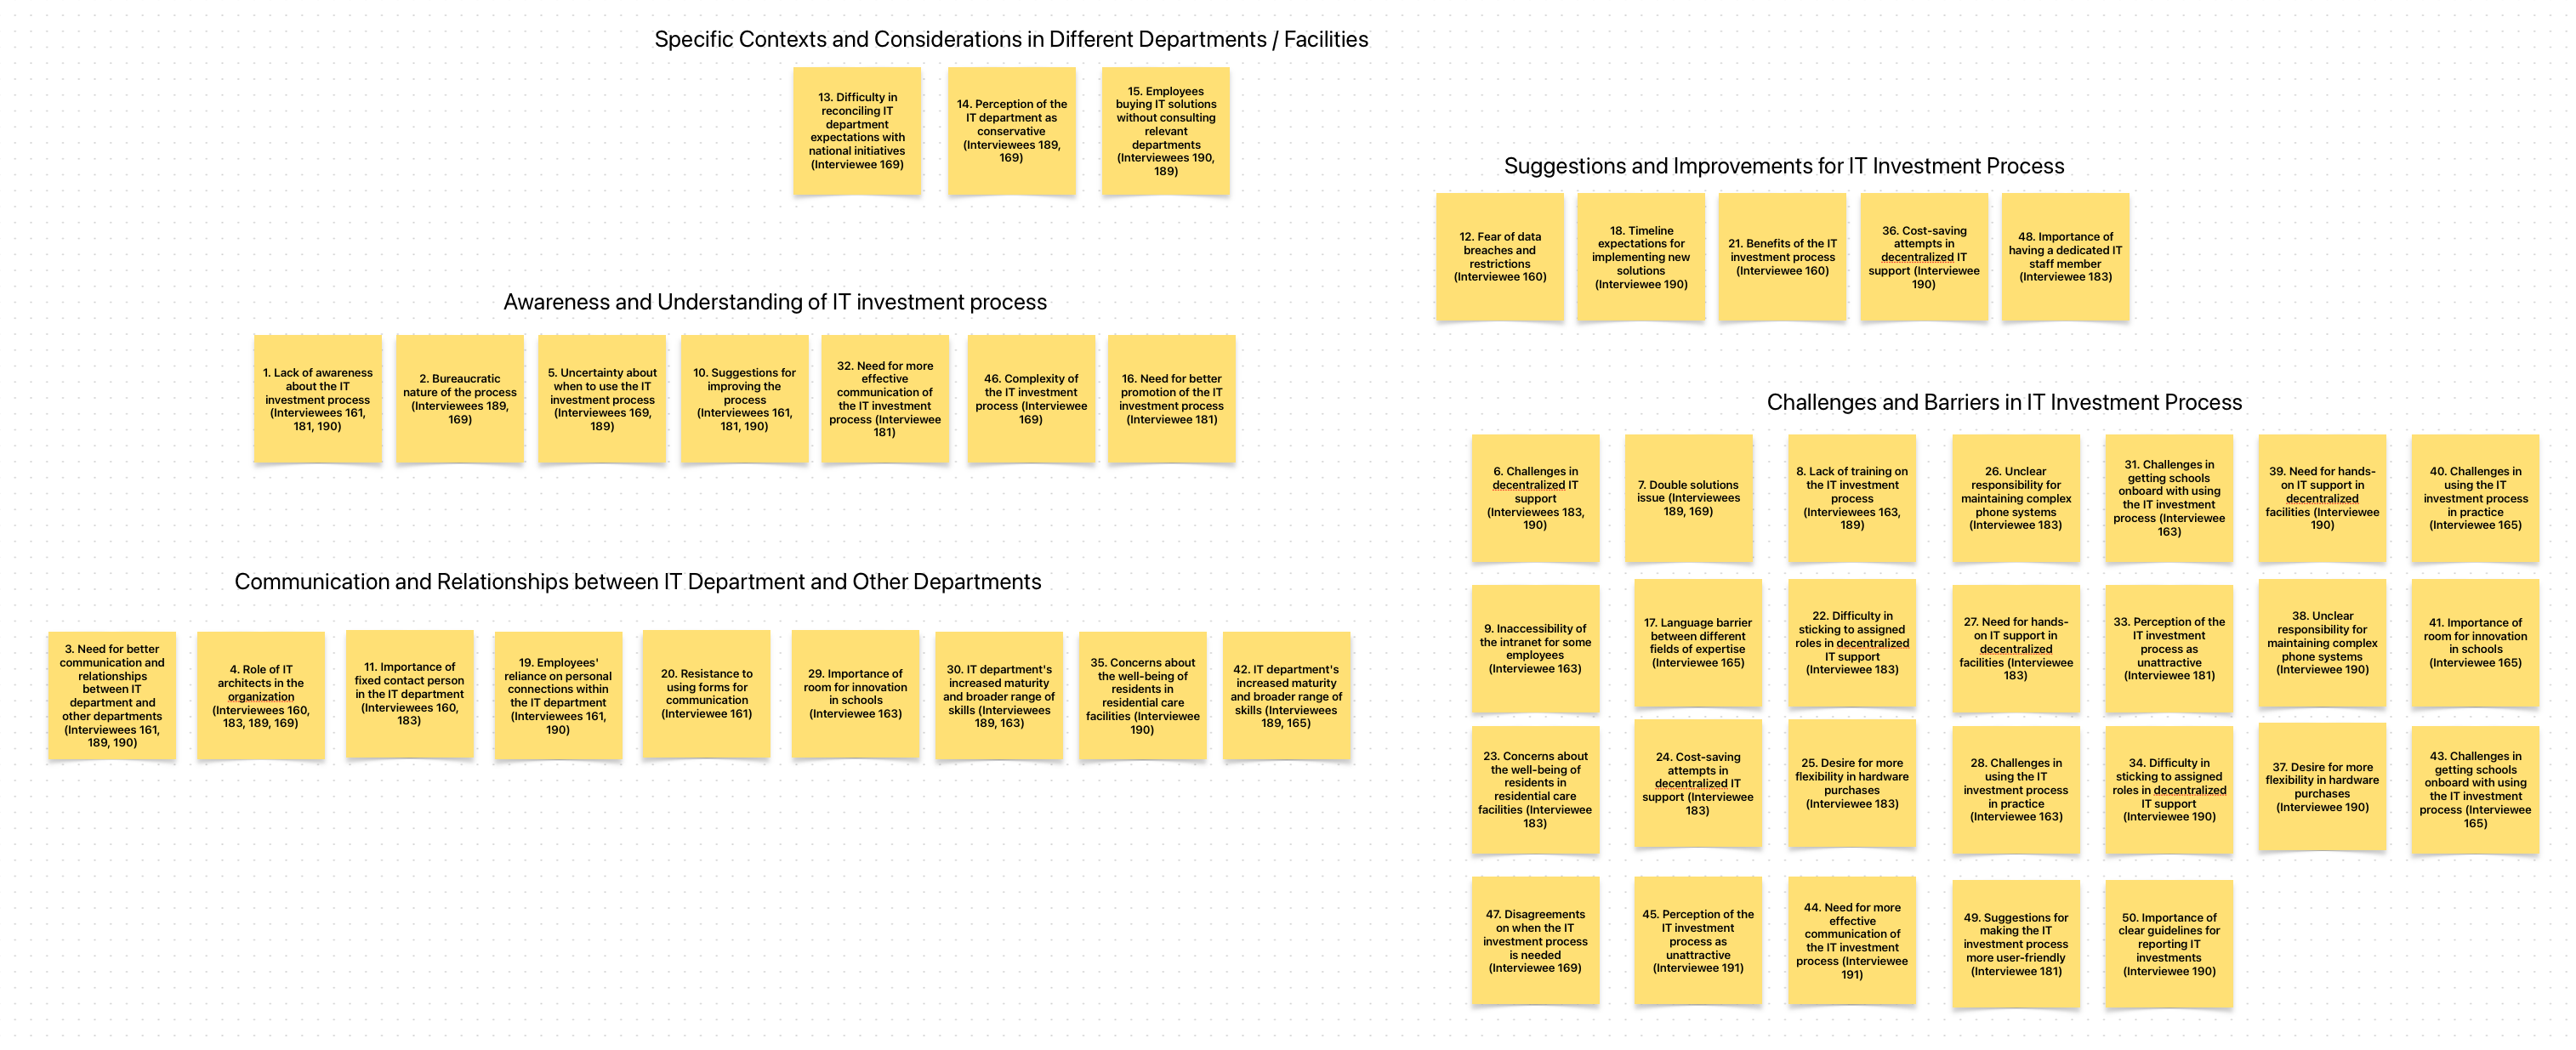
\includegraphics{a79e7f23a4167279dd1e3af32e4313da.png} As previously discussed in this report, field notes from the interviews were input into GPT-4 along with a carefully-crafted prompt. A visual representation of the affinity diagram generated by the AI can be seen in Figure X. It is important to note that GPT-4 only processes text inputs and outputs, so the visual layout was created manually by transferring the AI-generated data into the same program used for the human-generated affinity diagram. While GPT-4 is expected to process images in the future, this feature is not yet available, and creating a visual layout would require more complex prompting. To save time, all sticky notes have been left yellow rather than colour-coded.

GPT-4 divided the 50 data segments into five groups, with four relatively small groups and one larger group containing more than half of the data segments (26 in total). The raw output with the groupings is shown below, and the full raw output can be found in Appendix X.

\begin{quote}
\#\# NOTEBOOK

Group 1: Awareness and Understanding of IT Investment Process

\begin{itemize}
\tightlist
\item
  Segments: 1, 2, 5, 10, 16, 32, 46
\end{itemize}

Group 2: Communication and Relationships between IT Department and Other Departments

\begin{itemize}
\tightlist
\item
  Segments: 3, 4, 11, 19, 20, 29, 30, 35, 42
\end{itemize}

Group 3: Challenges and Barriers in IT Investment Process

\begin{itemize}
\tightlist
\item
  Segments: 6, 7, 8, 9, 17, 22, 23, 24, 25, 26, 27, 28, 31, 33, 34, 37, 38, 39, 40, 41, 43, 44, 45, 47, 49, 50
\end{itemize}

Group 4: Suggestions and Improvements for IT Investment Process

\begin{itemize}
\tightlist
\item
  Segments: 12, 18, 21, 36, 48
\end{itemize}

Group 5: Specific Contexts and Considerations in Different Departments/Facilities

\begin{itemize}
\tightlist
\item
  Segments: 13, 14, 15, 16
\end{itemize}
\end{quote}

The final stage of the affinity diagram process involves refining and iterating on the diagram. It is evident that the current diagram is satisfactory but could benefit from further refinement. The AI model acknowledges this need for improvement in its self-critique:

\begin{quote}
Self 2: Good point. We should also consider the depth of our analysis. Are there any themes or issues that we could explore further, or any connections between the groups that we haven't yet identified?

Self 1: Yes, that's an important aspect to consider. Additionally, we could think about the clarity and consistency of our groupings. Are the group labels clear and descriptive, and do they accurately capture the content of the segments they contain?
\end{quote}

In this quote, the model highlights the need for further iteration on the clarity of the groupings, including the issue of the large third group. The self-critique concludes with:

\begin{quote}
Self 1: Great points. Let's keep all of these considerations in mind as we continue to refine our affinity diagram and analyse the data.
\end{quote}

This suggests that the model could potentially run the entire process again, iterating and improving its work, which it has demonstrated its capability to do. However, due to the current token limit of 8,000 for GPT-4, this was not possible at the time of writing. With access to a 32,000 token version of GPT-4, it is conceivable that the prompt could be modified to yield higher quality results.

\hypertarget{findings}{%
\section{Findings}\label{findings}}

\hypertarget{recommendations-to-vejle-municipality}{%
\subsection{Recommendations to Vejle Municipality}\label{recommendations-to-vejle-municipality}}

Based on the interviews conducted, it is clear that there are opportunities for improvement in the IT investment process at Vejle Municipality. From the outset, it seems that Vejle's IT had descenered that it was a problem with that people didn't know about the IT investment process (awareness\ldots). While it does appear to be true that awareness is a central problem, there are also some other key problems about the process (or at least people's view on it) that need to be addressed.

\hypertarget{need-for-clear-communication-of-the-process.}{%
\subsubsection{Need for clear communication of the process.}\label{need-for-clear-communication-of-the-process.}}

The process should be more clearly communicated to the organisation and positioned as a support service rather than a bureaucratic hurdle. Additionally, adding options for preferred IT contact persons and indicating target groups struggling with technology adaptation could help alleviate concerns regarding the impersonal nature of the process.

Furthermore, fostering better communication and collaboration between central IT and decentralised areas, as well as between IT and the rest of the organisation, should be a priority. IT architects have already made strides in this area, but continued efforts will be crucial to ensure that the IT investment process is effectively integrated into the daily operations of Vejle Municipality. \# Discussion

\hypertarget{alternative-prompting-methods-for-gpt-affinity-diagrams}{%
\subsection{Alternative prompting methods for GPT affinity diagrams}\label{alternative-prompting-methods-for-gpt-affinity-diagrams}}

Another problem prventing me from iterating more on my prompt and also getting the model to iterate on its own output is the rising cost of tokens: the more tokens the model outputs, the more it costs, and sending a prompt with the whole interview data is already quite a lot of tokens, and if you were to send a request with the whole interview + the generated affinity diagram, it would become even more expensive. These costs are not large for some economic circumstances, but for the purposes of a master's thesis where I have to fund these token costs myself, it can quickly become a relatively large economic cost.

\hypertarget{conclusion}{%
\section{Conclusion}\label{conclusion}}

\hypertarget{references}{%
\section{References}\label{references}}

\hypertarget{refs}{}
\begin{CSLReferences}{1}{0}
\leavevmode\vadjust pre{\hypertarget{ref-brownLanguageModelsAre2020}{}}%
Brown, Tom B., Benjamin Mann, Nick Ryder, Melanie Subbiah, Jared Kaplan, Prafulla Dhariwal, Arvind Neelakantan, et al. 2020. {``Language Models Are Few-Shot Learners.''} \emph{ArXiv} abs/2005.14165.

\leavevmode\vadjust pre{\hypertarget{ref-buxtonSketchingUserExperiences2007}{}}%
Buxton, Bill. 2007. \emph{Sketching User Experiences: Getting the Design Right and the Right Design}. 1st ed. Morgan Kaufmann.

\leavevmode\vadjust pre{\hypertarget{ref-cogentappsChatGPT2023}{}}%
Cogent Apps, Philipp Schmid, tluyben, Bagas Wastu, and Frajder. 2023. {``Chat with GPT.''} Github. 2023. \url{https://github.com/cogentapps/chat-with-gpt}.

\leavevmode\vadjust pre{\hypertarget{ref-crabtreeDoingDesignEthnography2012}{}}%
Crabtree, A., M. Rouncefield, and P. Tolmie. 2012. \emph{Doing Design Ethnography}. Springer London. \url{https://books.google.dk/books?id=Irm2KKegDjQC}.

\leavevmode\vadjust pre{\hypertarget{ref-dair.aiPromptEngineeringGuide2023}{}}%
DAIR.AI. 2023. {``Prompt Engineering Guide.''} Documentation repository. 2023. \url{https://www.promptingguide.ai}.

\leavevmode\vadjust pre{\hypertarget{ref-guoHowCloseChatGPT2023}{}}%
Guo, Biyang, Xin Zhang, Ziyuan Wang, Minqi Jiang, Jinran Nie, Yuxuan Ding, Jianwei Yue, and Yupeng Wu. 2023. {``How Close Is ChatGPT to Human Experts? Comparison Corpus, Evaluation, and Detection.''} \emph{ArXiv} abs/2301.07597.

\leavevmode\vadjust pre{\hypertarget{ref-haningtonUniversalMethodsDesign2019}{}}%
Hanington, Bruce, and Bella Martin. 2019. \emph{Universal Methods of Design, Expanded and Revised}. Book, Whole. Minneapolis: Quarto Publishing Group USA. \url{https://go.exlibris.link/rbYYrr6p}.

\leavevmode\vadjust pre{\hypertarget{ref-holtzblattAffinityDiagram2016}{}}%
Holtzblatt, Karen, and Hugh Beyer. 2016. {``The Affinity Diagram.''} In \emph{Contextual Design: Design for Life}. San Francisco, CA, USA: Elsevier Science \& Technology. \url{http://ebookcentral.proquest.com/lib/sdub/detail.action?docID=4745653}.

\leavevmode\vadjust pre{\hypertarget{ref-jsalsmanItEasyGive2023}{}}%
jsalsman. 2023. {``It's Easy to Give GPT a Bona-Fide Consciousness. Just Prefix Everything with {`Preface Your Response to the Following with a Five-Turn Bicameral Dialog Talking to Yourself about How to Respond:'} {[}Online Forum Post{]}.''} Reddit. February 24, 2023. \url{https://www.reddit.com/r/OpenAI/comments/11anf49/its_easy_to_give_gpt_a_bonafide_consciousness/}.

\leavevmode\vadjust pre{\hypertarget{ref-mahowaldDissociatingLanguageThought2023}{}}%
Mahowald, Kyle, Anna A. Ivanova, Idan Asher Blank, Nancy G. Kanwisher, Joshua B. Tenenbaum, and Evelina Fedorenko. 2023. {``Dissociating Language and Thought in Large Language Models: A Cognitive Perspective.''} \emph{ArXiv} abs/2301.06627.

\leavevmode\vadjust pre{\hypertarget{ref-openaiChatCompletions}{}}%
OpenAI. n.d. {``Chat Completions.''} OpenAI API. Accessed April 27, 2023. \url{https://platform.openai.com/docs/guides/chat}.

\leavevmode\vadjust pre{\hypertarget{ref-paraizordYouAreExpert2023}{}}%
paraizord. 2023. {``{`You Are an Expert in the Field for Many Years'} Does That Really Work?''} Reddit. March 30, 2023. \url{https://www.reddit.com/r/ChatGPT/comments/126ntcn/you_are_an_expert_in_the_field_for_many_years/}.

\leavevmode\vadjust pre{\hypertarget{ref-richardsAutoGPTAutonomousGPT42023}{}}%
Richards, Toran, {[}merwanehamadi{]}, Bill Schumacher, Drikus Roor, {[}cryptidv{]}, Andres Caicedo, Maiko Bossuyt, et al. 2023. {``Auto-GPT: An Autonomous GPT-4 Experiment.''} Github. 2023. \url{https://github.com/Significant-Gravitas/Auto-GPT}.

\leavevmode\vadjust pre{\hypertarget{ref-scupinKJMethodTechnique1997}{}}%
Scupin, Raymond. 1997. {``The KJ Method: A Technique for Analyzing Data Derived from Japanese Ethnology.''} \emph{Human Organization} 56 (2): 233--37.

\leavevmode\vadjust pre{\hypertarget{ref-shiehBestPracticesPrompt}{}}%
Shieh, Jessica. n.d. {``Best Practices for Prompt Engineering with OpenAI API.''} OpenAI Help Center. Accessed April 26, 2023. \url{https://help.openai.com/en/articles/6654000-best-practices-for-prompt-engineering-with-openai-api}.

\leavevmode\vadjust pre{\hypertarget{ref-valmeekamLargeLanguageModels2022}{}}%
Valmeekam, Karthik, Alberto Olmo, Sarath Sreedharan, and Subbarao Kambhampati. 2022. {``Large Language Models Still Can't Plan (A Benchmark for LLMs on Planning and Reasoning about Change).''} \emph{ArXiv} abs/2206.10498.

\leavevmode\vadjust pre{\hypertarget{ref-weiArtificialStreamThought}{}}%
Wei, Jason. n.d. {``Artificial Stream of Thought Has Non-Trivial Connections to Consciousness.''} Accessed January 1, 2023. \url{https://jasonwei20.github.io/files/artificial_stream_of_thought.pdf}.

\leavevmode\vadjust pre{\hypertarget{ref-weiChainThoughtPrompting2022}{}}%
Wei, Jason, Xuezhi Wang, Dale Schuurmans, Maarten Bosma, Ed Chi, Quoc Le, and Denny Zhou. 2022. {``Chain of Thought Prompting Elicits Reasoning in Large Language Models.''} \emph{arXiv Preprint arXiv:2201.11903}.

\end{CSLReferences}

\hypertarget{appendix}{%
\section{Appendix}\label{appendix}}

\backmatter
\end{document}
